%\documentclass[a4paper,12pt,oneside,draft]{article}
\documentclass[a4paper,12pt,oneside]{article}

% In the original writelatex tamplate
\usepackage[english]{babel}
\usepackage[utf8]{inputenc}
\usepackage{amsmath}
\usepackage{graphicx}

% By LoCigno
\usepackage{times}
\usepackage{graphicx}
\usepackage{subfigure}
\usepackage{color}
\usepackage{url}
\usepackage{cleveref}

% By Davide
\usepackage{comment}
\usepackage{booktabs}
\usepackage{color}

%Variables macros
\newcommand{\DefineVar}[2]{%
  \expandafter\newcommand\csname var-#1\endcsname{#2}%
} 
\newcommand{\var}[1]{\csname var-#1\endcsname}

\usepackage{courier}
\newcommand{\mono}[1]{\texttt{#1}}
%\newcommand{\mono}[1]{\texttt{\textbf{#1}}}

\title{Identification procedure for Lego Mindstorm motor}

\author{Diego Verona, Aliaksandr Siarohin, Mattia Digilio}

\date{\today}

\begin{document}
%\maketitle
\makeatletter  % populates \@title, \@author, \@date
\begin{titlepage}
      \centering
      ~~~~~~~~~~~~~\\[-30mm]
      
\includegraphics[keepaspectratio=true, width=7cm]{bg_eng_1r.jpg} \\[10mm]

     {
     \large \bfseries Master Degree in Computer Science\\[3mm] 
     Applied Robotics\\[3mm]
     AA 2015-2016
     }\\[10mm]

     %--------------------------------
     % Set the title, author, and date
     % 

     \vspace{0.5cm}
     {
     \Large \bfseries \textcolor{blue}{\@title} \par
     }
     \vspace{0.5cm}
%      {
%      \large {Group N. 1} \par
%      }
     \vspace{0.2cm}

     {\large {\@author}}
     \\ \vspace{.2cm}
     \@date

     \vspace{0.6cm}

    %-----------------------------------

\begin{abstract}

\textit{
  Report for the first assignment on Applied robotics: getting and identification parameters of the Lego NXT motors.\\In this report we discuss our method of obtaining data from Lego Mindstorm motors as well as estimation of parameters from the motor  data.
}


\end{abstract}

\end{titlepage}


\section{Tools and definitions}
\subsection{General definition}
..
\subsection{Used tools}
..

\section{Collecting motor data}
Have been used 2 different methods to collect motor data:
\begin{enumerate}
\item Bluetooth connection
\item Usb connection
\end{enumerate}
It is important get the minimum time gap between measures, but it require an extra check to detect if the tachometer sensor is fast and precious as the used transmission.
For this report is decider to use USB connection getting 10 different data files with different raw powers.
\subsection{Bluetooth data collection}
Given by the lab the code to comunicate between our PC and the NXT brick, we learned how it works and we implement the interface to include also the current measure NXT timestamp. The procedure to get data with bluetooth is the following:
\begin{enumerate}
\item Send message from PC to brick that set motor power
\item Send message from PC to brick that requests tachometer count from the motor
\item Receive message from brick with tachometer count and relative timestamps
\item Save timestamps and tachometer count to file
\item Repeat all from step 2
\end{enumerate}
Using this methodology there is a very hight latency $\approx 50ms$. It is possible to force the speed connection, but using USB connection it results more reliable and fast.
Code is available here: \url{https://github.com/AliaksandrSiarohin/AppliedRobotics/brofist}
\subsection{USB data collection}
To establish a connection between PC and NXT brick is possible using a specific Pyton library called "pyusb".
The procedure to get data with this method is the following:
\begin{enumerate}
\item Establish connection with brick using pyusb
\item Set up the motor power on the brick
\item Send (timestamp,  tacho count) from PC to brick
\item Receive (timestamp,  tacho count)from brick to PC
\item Save collected data to file
\item Go to step 3
\end{enumerate}
Using this methodology is possible to obtain much better performance about $\approx 2ms$ latency. 
Code is available here: \url{https://github.com/AliaksandrSiarohin/AppliedRobotics/usb_collector}
\section {Estimating the parameters from the data}
To estimate the parameters we filter the data using butterworth filter and then we estimate the parameters using 2 methods:
\begin{itemize}
\item Regular method proposed on the lecture
\item Regression method
\end{itemize}

\subsection {Filtering}
We use butterwoth filter of order 1 and and cut-off frequency 0.02. For example \cref{fig:filterd}.
\begin{figure}[t]%
	\centering
	%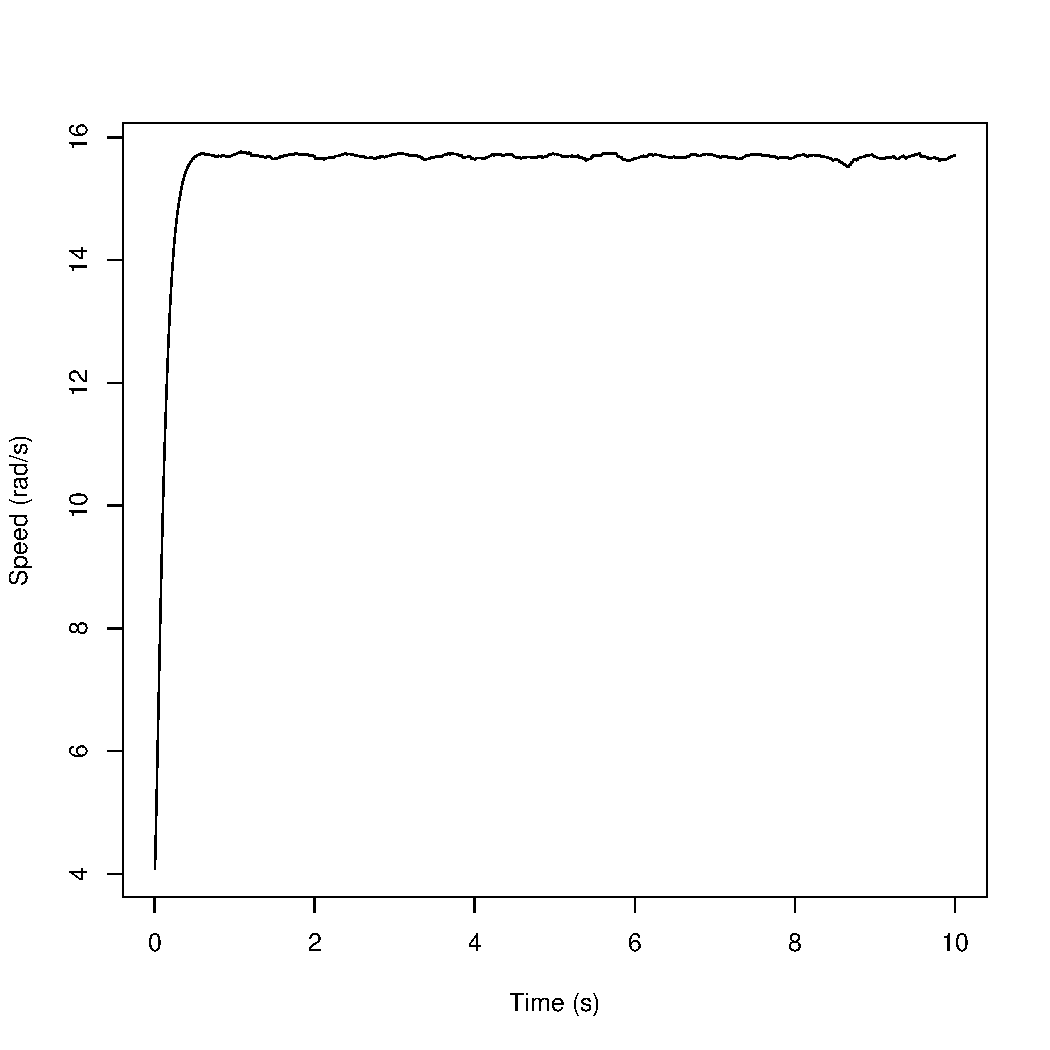
\includegraphics[width=\columnwidth]{~/apr/AppliedRobotics/motor_data/plots/v90_20000.pdf}
	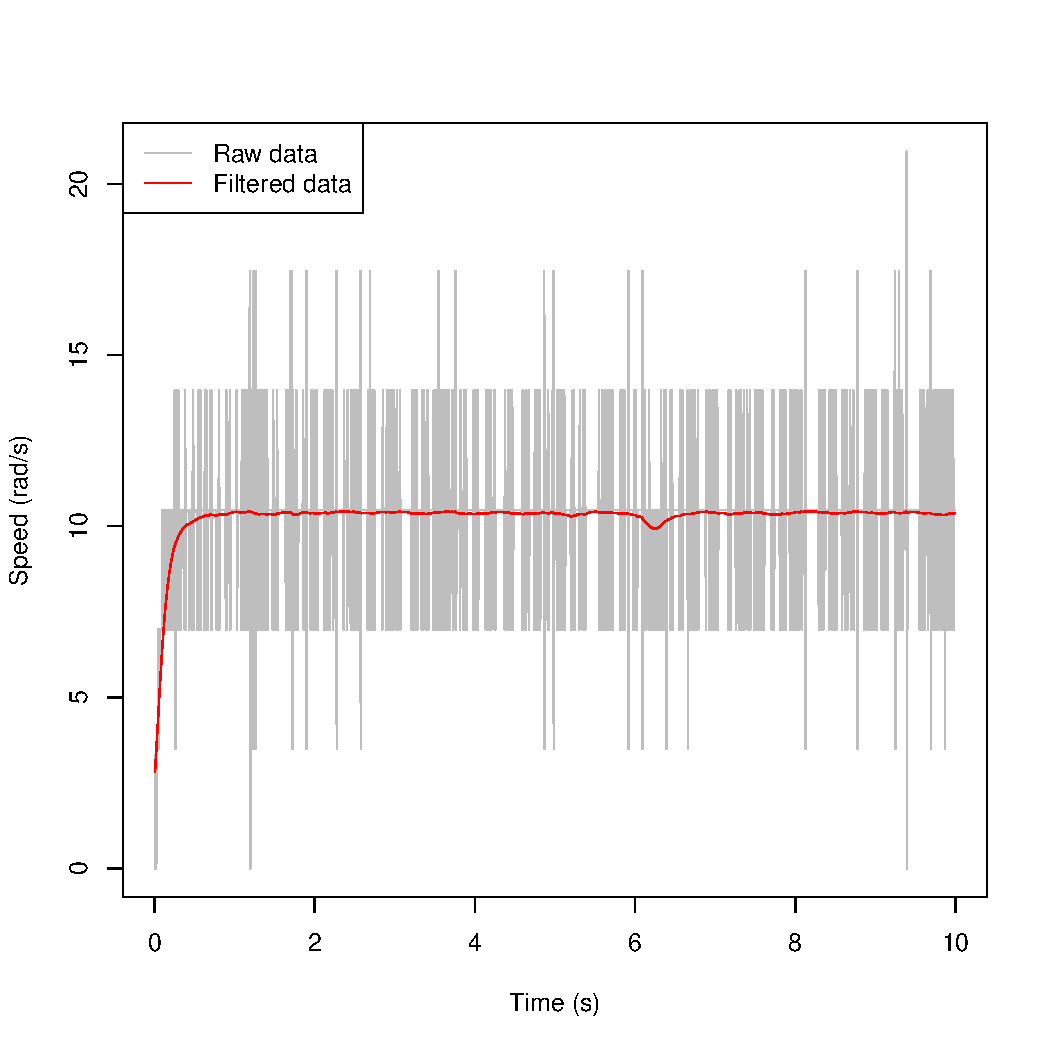
\includegraphics[width=\columnwidth]{C:/Users/Diego/Desktop/NXT/motor_data/plots/filtering/60.pdf}
	\caption{Deviation of x from it`s mean.}%
	\label{fig:filtered}%
\end{figure}


\end{document}